\documentclass[oneside, landscape, twocolumn, a4wide, 9pt]{scrartcl}
\usepackage{savetrees}
\usepackage{bera}
\usepackage[brazilian]{babel}
\usepackage[utf8x]{inputenc}
\usepackage{epsfig}
\usepackage{amsmath}
\usepackage{amssymb}
\usepackage{amsthm}
\usepackage{graphicx}
\usepackage{pstricks}
\usepackage{cancel}
\usepackage{tocloft}
\usepackage{titlesec}
\usepackage{fancyvrb}
\usepackage{pdfpages}
\usepackage{fancyhdr}

\setlength{\columnsep}{.25in}
\setlength{\columnseprule}{.25pt}
\parindent=0in

\setcounter{tocdepth}{1}

\renewcommand{\cftbeforesecskip}{0cm}

\fvset{fontsize=\small}

\titleformat{\section}
{\titlerule
\vspace{0.1cm}%
\normalfont\bf\itshape}
{\thesection.}{.5em}{}

\DefineShortVerb{\|}

\pagestyle{fancyplain}
\renewcommand{\headrulewidth}{.25pt}
\fancyhf{}
\lhead{\Huge\sf [ITA] Carteado}
\chead{}
\rhead{\Huge\sf\thepage}
\lfoot{}
\cfoot{}
\rfoot{}

\begin{document}
\tableofcontents
\thispagestyle{fancyplain}

\section{Codigos de início de prova}
\subsection{Makefile}
\VerbatimInput{Makefile.txt}
\subsection{modelo.cpp}
\VerbatimInput{modelo.cpp}
\subsection{shell}
\VerbatimInput{struct.sh}

\section{Bugs do Milênio}

\begin{itemize}
	\item Leu o enunciado direito? Pediu clarifications?
	\item Criar casos de teste
	\item Verificar overflows, ver se o $\infty$ é tão infinito quanto parece
	\item Doubles: igualdade com tolerância
	\item Igualdade dentro de |if|
	\item |C-w C-y|? Errou algo.
	\item Tamanho de vetores
	\item |long long a = 1 << 40;| $\Longrightarrow$ |long long a = 1ll << 40;| %>>>>
	\item Variáveis com nome min, max, next
	\item Inicialização de variáveis
	\item Casos extremos, muito pequenos ou muito grandes, caso zero
	\item Self-loops e multiarestas em grafos
	\item Otimização de casos específicos
	\item Imprecisão ao subtrair números quase iguais
	\item Resto de divisão com números negativos
\end{itemize}

\section{Geometria (números inteiros)}

\VerbatimInput{geometria-inteiros.cpp}

\section{Geometria (ponto flutuante)}

\VerbatimInput{geometria-doubles.cpp}

\section{Teoria dos Números}
\VerbatimInput{ntheory.cpp}

\section{Garfos}

\VerbatimInput{grafos.cpp}

\section{BigNum}

\VerbatimInput{bignum.cpp}

\section{Álgebra Linear}

\VerbatimInput{alglin.cpp}

\section{Strings}

\VerbatimInput{strings.cpp}

\section{Binary Indexed Tree}

\VerbatimInput{bit.cpp}

\section{Interval Tree}

\VerbatimInput{intervaltree.cpp}

\section{Problemas}

\VerbatimInput{problemas.cpp}

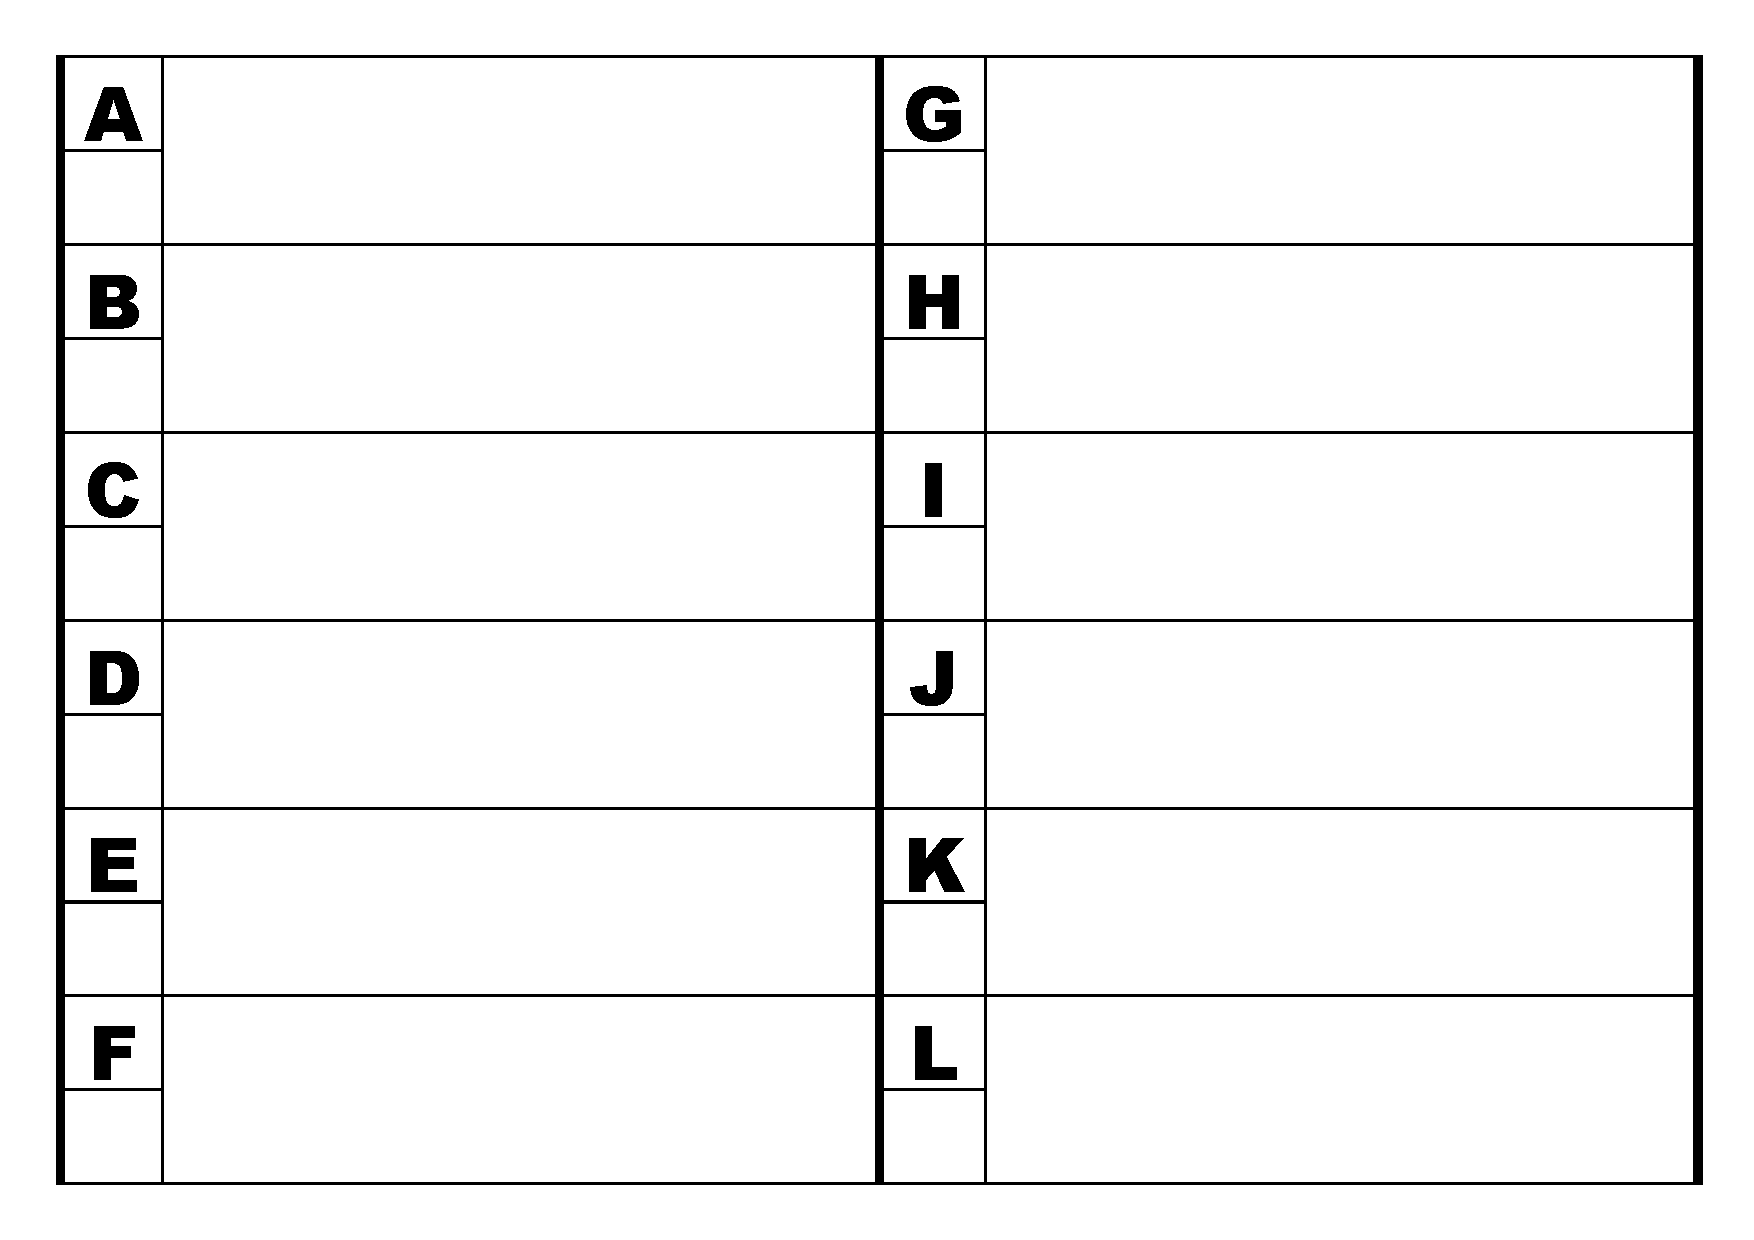
\includepdf[pages=1]{status-v2}

\end{document}
